% vim:ft=tex:ts=2:sw=0
% Author: Plump Albert (plumpalbert@gmail.com)
\documentclass[../nirs.tex]{subfiles}
\usepackage[figuresleft]{rotating}

\begin{document}
\section{Выявление основных понятий и процессов, их свойств и закономерностей.
Построение ER-диаграммы предметной области}

\subsection{Основные понятия}
Техническое обслуживание (ТО) -- это комплекс организационно-технических мероприятий
и работ, производимых на объекте и направленных на поддержание в рабочем или
исправном состоянии оборудования технических систем в процессе их использования
по назначению, с целью повышения надежности и эффективности их работы
[\ref{ref:техническое-обслуживание}].

Текущий ремонт (ТР) -- устранение мелких неисправностей и отказов автомобиля.
Способствует выполнению установленных норм пробега автомобиля до капитального
ремонта. Текущий ремонт заключается в проведении разборочно-сборочных,
слесарных, сварочных и других работ, а также в замене деталей в автомобиле
(прицепе, полуприцепе) [\ref{ref:му-ремонт-и-техническое-обслуживание}].

Календарное планирование -- распределение во времени видов деятельности.
Календарное планирование представляет собой составление на основе календаря
таблицы, в которой по датам расписаны мероприятия, которые нужно провести либо
принять в них участие.
Планирование бывает персональным или групповым.
В групповом планировании определяемые мероприятия и действия должны быть
согласованы группой участников.
Составляемые планы могут быть закрытыми для посторонних лиц, либо открытыми, где
они играют роль объявлений [\ref{ref:календарное-планирование}].

\subsection{Основные процессы}
Разрабатываемая информационная система должна обеспечивать выполнение следующих
бизнес-процессов:
\begin{itemize}
  \item обеспечивать просмотр и редактирование информации о конкретном
    автомобиле;
  \item обеспечивать просмотр и редактирование информации о текущем статусе
    работ;
  \item обеспечивать просмотр и редактирование информации о сотрудниках;
  \item обеспечивать просмотр и редактирование информации о доступных на
    складе ресурсах;
  \item прогнозировать дату окончания выполнения работ;
  \item составлять график прохождения технического обслуживания и ремонта
    техникой.
\end{itemize}

\subsection{Построение ER-диаграммы предметной области}
В автоматизированных информационных системах отражение предметной области
представлено моделями данных нескольких уровней:
\begin{enumerate}
  \item Инфологический.
  \item Даталогический.
  \item Физический.
\end{enumerate}

На каждом уровне проводится структуризация информации таким образом, чтобы на
третьем уровне информация могла быть представлена в виде структур данных,
реализуемых в памяти ЭВМ.

В результате исследования предметной области строится ее инфологическая модель,
которая описывается в терминах классов объектов и их взаимодействий. В
инфологической модели определяется какая информация о предметной области будет
хранится и обрабатываться в компьютере. Информация представляется вне
зависимости от того, что представляют собой данные и какие технические средства
будут использовании в дальнейшем для ее хранения и обработки. Цель инфологического
проектирования заключается в представлении семантики (смысла) предметной
области. Для описания предметной области наиболее часто используется модель
\textquote{сущность–связь}, которую сокращенно называют ER–моделью от
английского названия \textquote{Entity – Relationship} (\textquote{Сущность –
связь}). ER–диаграмма модели имеет лексикографическую структуру и включает в
себя текст и элементы графики [\ref{ref:er-диаграммы}].

При проектировании структуры предметной области определяют сущности (объекты,
явления), которые должны найти свое отражение в будущей системе.
Цель инфологического этапа проектирования состоит в получении семантических
(концептуальных) моделей, отражающих предметную область и информационные
потребности пользователей.

Классовая диаграмма разрабатываемой системы представлена на рисунке
\ref{fig:2_1_er_diagram}.

\begin{sidewaysfigure}[hp!]
  \centering
  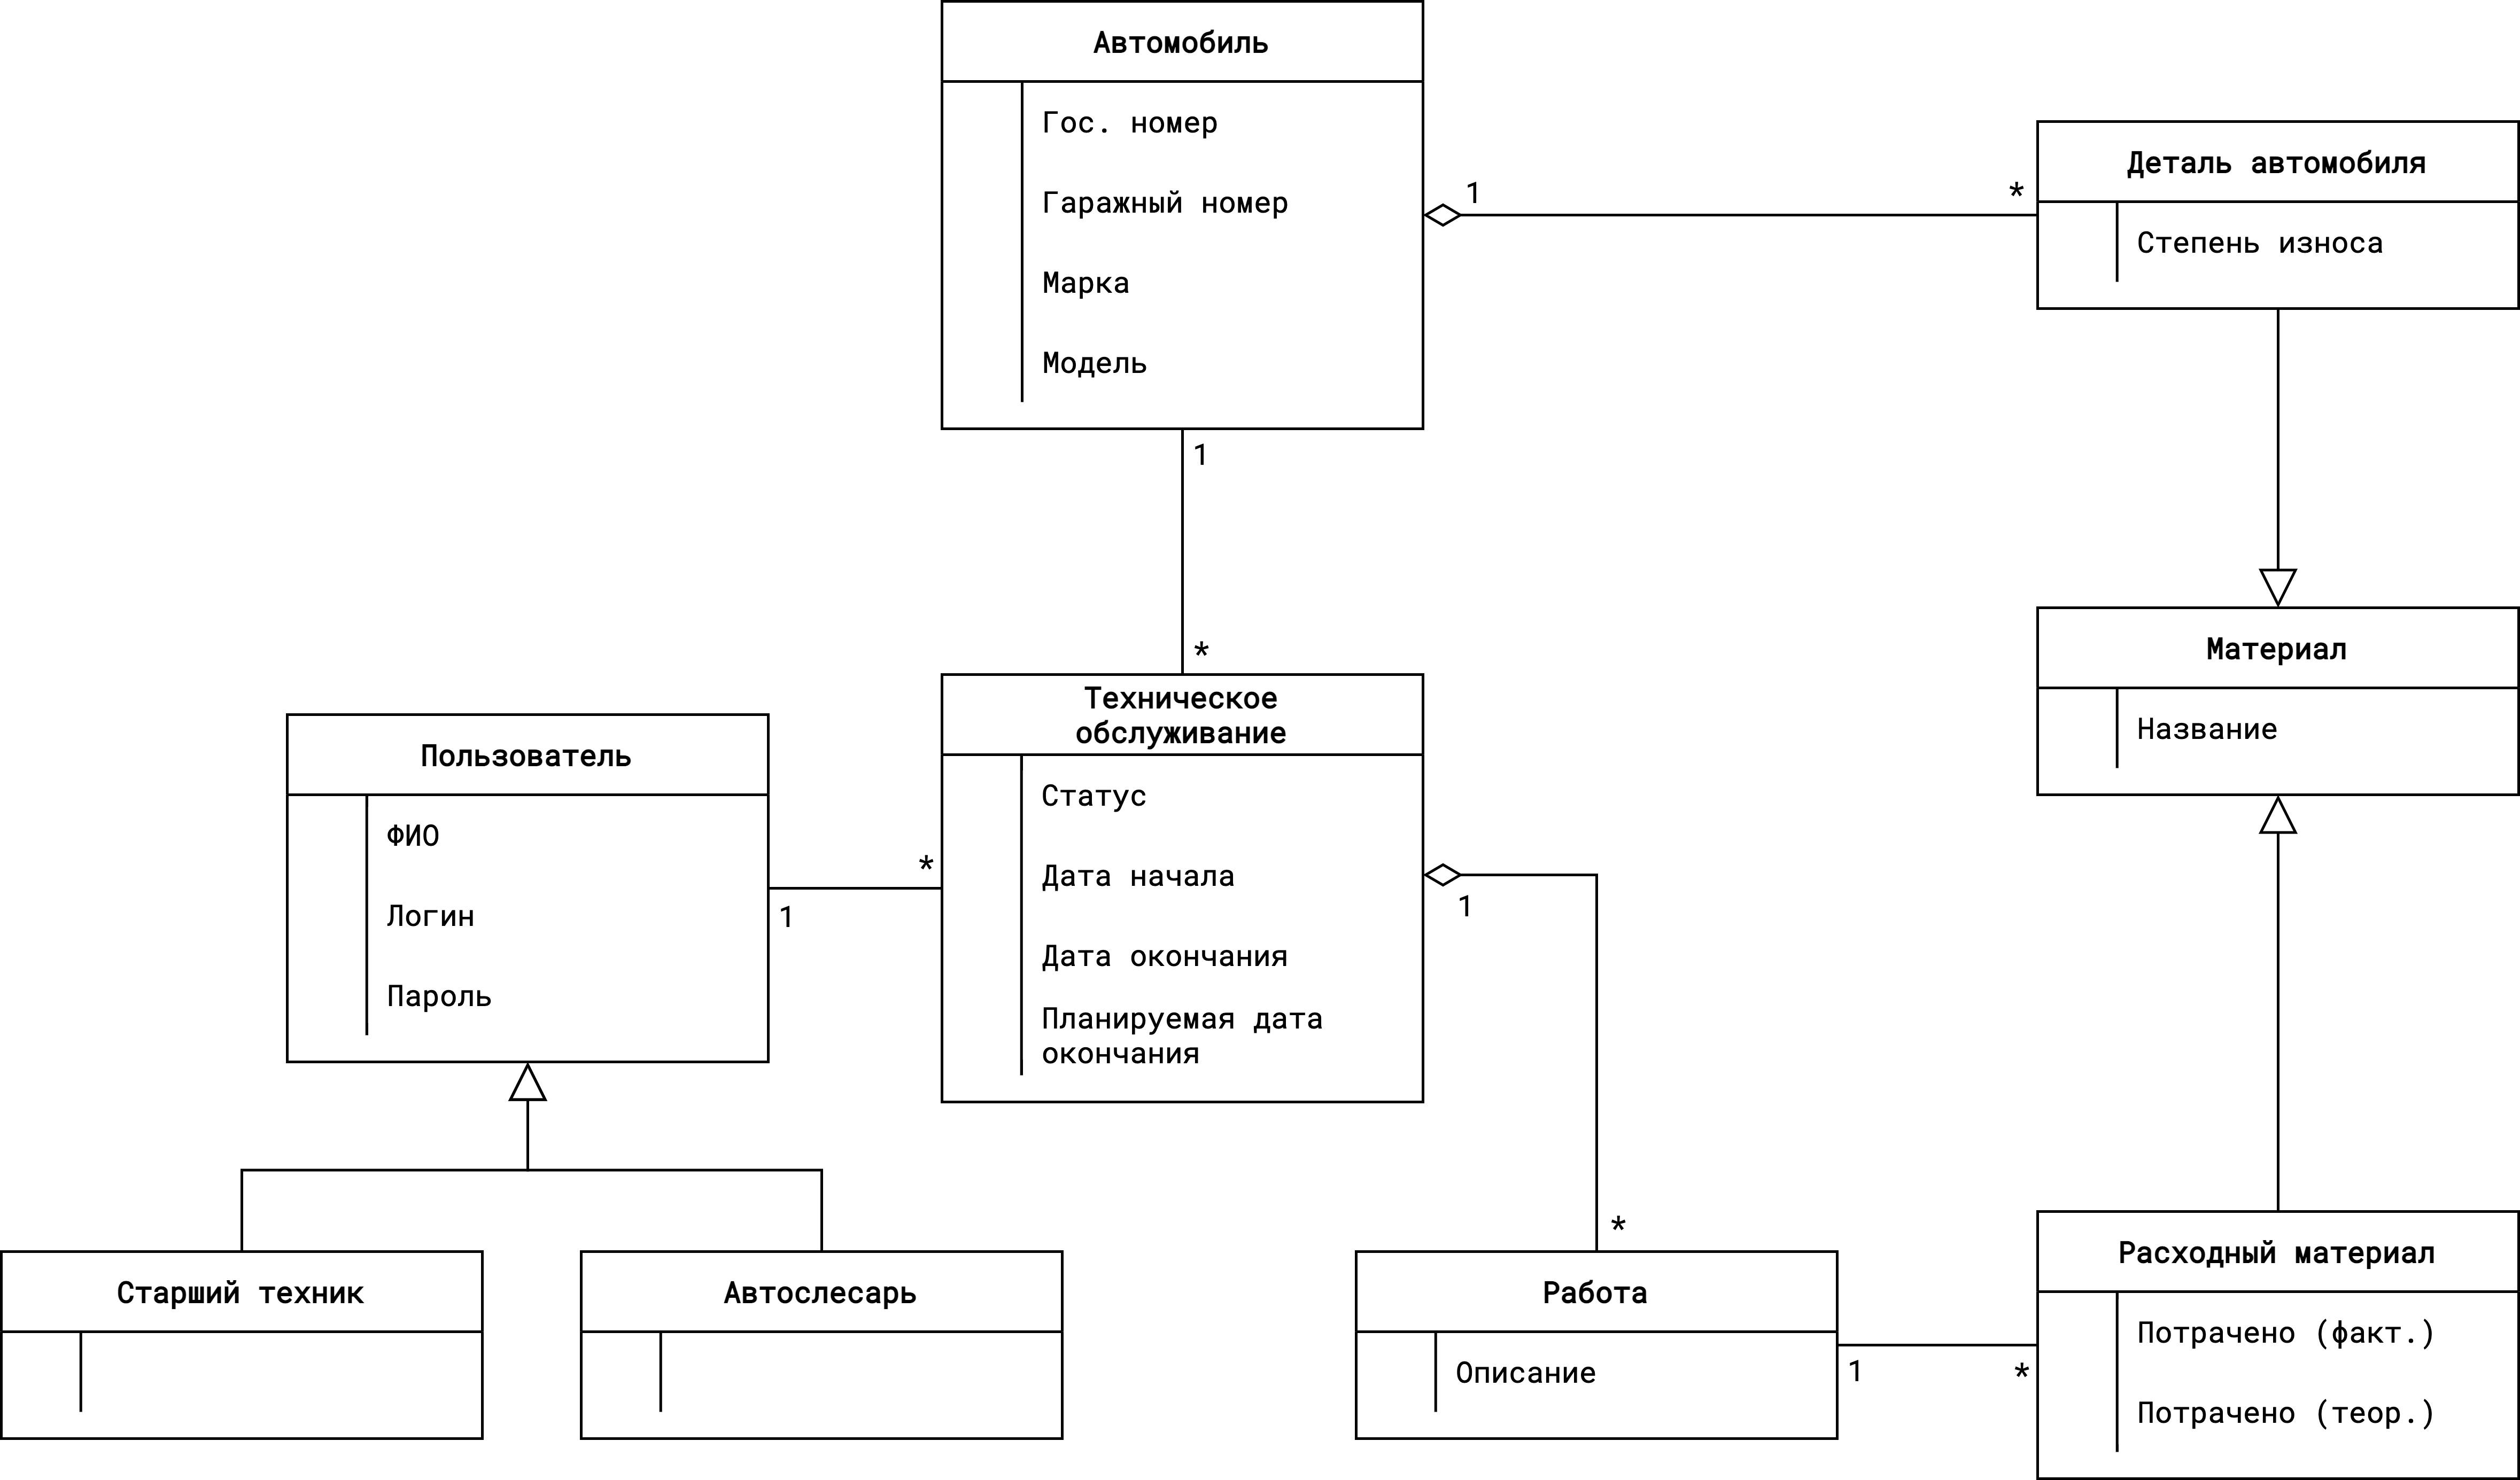
\includegraphics[keepaspectratio,
                   width=\textwidth,
                   height=0.6\textheight]{./images/er-diagram.drawio.png}
  \caption{ER-диаграмма системы}
  \label{fig:2_1_er_diagram}
\end{sidewaysfigure}

\pagebreak

Центральной сущностью, представляющей основной интерес разрабатываемой системы,
является \textquote{Автомобиль}. Она содержит информацию о конкретной единице
техники, такую как государственный регистрационный номер, гаражный номер, марка
и модель автомобиля.

Автомобиль состоит из запчастей (колесо, рулевое реле и пр.) и материалов
(двигательное масло, тормозная жидкость и пр.). В системе они объединены в одну
сущность -- \textquote{Материал}. Она содержит код материала и его наименование.
Помимо этого связь между сущностями \textquote{Автомобиль} и
\textquote{Материал} содержит дополнительный атрибут -- степень износа.

Одним из пользователей системы является старший техник. В разрабатываемой
системе он выступает в качестве сущности \textquote{Старший техник}, содержащей
имя сотрудника.

Задачей старшего техника является календарное планирование прохождения
технического обслуживания автомобильной техникой. Сущность \textquote{График
прохождения ТО} состоит из множества работ, которые необходимо провести на
технике. Сущность \textquote{Техническое обслуживание} содержит информацию о
статусе проведения работ, их перечень, ожидаемые и реальные сроки их завершения.
На их выполнение требуется определенное количество материалов, что на диаграмме
отражено связью между сущностями \textquote{Техническое обслуживание} и
\textquote{Материал}. Она содержит предполагаемый и фактические расходы
материала, для проведения данных работ.

На каждое техническое обслуживание старший техник назначает исполнителя --
сущность \textquote{Автослесарь}, содержащую имя сотрудника.

\end{document}
